%%%%%%%%%%%%%%%%%%%%%%%%%%%%%%%%%%%%%%%%%
% Important note:
% Chapter heading images should have a 2:1 width:height ratio,
% e.g. 920px width and 460px height.
%
%%%%%%%%%%%%%%%%%%%%%%%%%%%%%%%%%%%%%%%%%


%----------------------------------------------------------------------------------------
%	PACKAGES AND OTHER DOCUMENT CONFIGURATIONS
%----------------------------------------------------------------------------------------

\documentclass[openany,11pt,fleqn]{book} % Default font size and left-justified equations

\usepackage[top=3cm,bottom=3cm,left=3.2cm,right=3.2cm,headsep=10pt,letterpaper]{geometry} % Page margins

\usepackage{xcolor} % Required for specifying colors by name
\definecolor{ocre}{RGB}{52,177,201} % Define the orange color used for highlighting throughout the book

% Font Settings
\usepackage{avant} % Use the Avantgarde font for headings
%\usepackage{times} % Use the Times font for headings
\usepackage{mathptmx} % Use the Adobe Times Roman as the default text font together with math symbols from the Sym­bol, Chancery and Com­puter Modern fonts
\usepackage{microtype} % Slightly tweak font spacing for aesthetics
\usepackage[utf8]{inputenc} % Required for including letters with accents
\usepackage[T1]{fontenc} % Use 8-bit encoding that has 256 glyphs
\usepackage{amsthm}

\usepackage{mathtools}

\usepackage{minted}

\usepackage{tikz}
\usepackage{pgfplots}
\usepgfplotslibrary{fillbetween}
\usepackage{multirow}
\usepackage{array}
\usetikzlibrary{arrows.meta, positioning, calc, trees, shapes, decorations, matrix, fit}

% Bibliography
\usepackage[style=alphabetic,sorting=nyt,sortcites=true,autopunct=true,babel=hyphen,hyperref=true,abbreviate=false,backref=true,backend=biber]{biblatex}
\addbibresource{bibliography.bib} % BibTeX bibliography file
\defbibheading{bibempty}{}
\usepackage{float}


%----------------------------------------------------------------------------------------
%	VARIOUS REQUIRED PACKAGES
%----------------------------------------------------------------------------------------

\usepackage{titlesec} % Allows customization of titles

\usepackage{graphicx} % Required for including pictures
\graphicspath{{Pictures/}} % Specifies the directory where pictures are stored
% \graphicspath{{Plots/}}
\usepackage{lipsum} % Inserts dummy text

\usepackage{tikz} % Required for drawing custom shapes

\usepackage[english]{babel} % English language/hyphenation

\usepackage{enumitem} % Customize lists
\setlist{nolistsep} % Reduce spacing between bullet points and numbered lists

\usepackage{booktabs} % Required for nicer horizontal rules in tables

\usepackage{eso-pic} % Required for specifying an image background in the title page

%----------------------------------------------------------------------------------------
%	MAIN TABLE OF CONTENTS
%----------------------------------------------------------------------------------------

\usepackage{titletoc} % Required for manipulating the table of contents

\contentsmargin{0cm} % Removes the default margin
% Chapter text styling
\titlecontents{chapter}[1.25cm] % Indentation
{\addvspace{15pt}\large\sffamily\bfseries} % Spacing and font options for chapters
{\color{ocre!60}\contentslabel[\thecontentslabel]{2cm}\color{ocre}} % Chapter number
{}  
{\color{ocre!60}\normalsize\sffamily\bfseries\;\titlerule*[.5pc]{.}\;\thecontentspage} % Page number
% Section text styling
\titlecontents{section}[1.25cm] % Indentation
{\addvspace{5pt}\sffamily\bfseries} % Spacing and font options for sections
{\contentslabel[\thecontentslabel]{1.25cm}} % Section number
{}
{\sffamily\hfill\color{black}\thecontentspage} % Page number
[]
% Subsection text styling
\titlecontents{subsection}[1.25cm] % Indentation
{\addvspace{1pt}\sffamily\small} % Spacing and font options for subsections
{\contentslabel[\thecontentslabel]{1.25cm}} % Subsection number
{}
{\sffamily\;\titlerule*[.5pc]{.}\;\thecontentspage} % Page number
[] 

%----------------------------------------------------------------------------------------
%	MINI TABLE OF CONTENTS IN CHAPTER HEADS
%----------------------------------------------------------------------------------------

% Section text styling
\titlecontents{lsection}[0em] % Indendating
{\footnotesize\sffamily} % Font settings
{}
{}
{}

% Subsection text styling
\titlecontents{lsubsection}[.5em] % Indentation
{\normalfont\footnotesize\sffamily} % Font settings
{}
{}
{}
 
%----------------------------------------------------------------------------------------
%	PAGE HEADERS
%----------------------------------------------------------------------------------------

\usepackage{fancyhdr} % Required for header and footer configuration

\pagestyle{fancy}
\renewcommand{\chaptermark}[1]{\markboth{\sffamily\normalsize\bfseries\chaptername\ \thechapter.\ #1}{}} % Chapter text font settings
\renewcommand{\sectionmark}[1]{\markright{\sffamily\normalsize\thesection\hspace{5pt}#1}{}} % Section text font settings
\fancyhf{} \fancyhead[LE,RO]{\sffamily\normalsize\thepage} % Font setting for the page number in the header
\fancyhead[LO]{\rightmark} % Print the nearest section name on the left side of odd pages
\fancyhead[RE]{\leftmark} % Print the current chapter name on the right side of even pages
\renewcommand{\headrulewidth}{0.5pt} % Width of the rule under the header
\addtolength{\headheight}{2.5pt} % Increase the spacing around the header slightly
\renewcommand{\footrulewidth}{0pt} % Removes the rule in the footer
\fancypagestyle{plain}{\fancyhead{}\renewcommand{\headrulewidth}{0pt}} % Style for when a plain pagestyle is specified

% Removes the header from odd empty pages at the end of chapters
\makeatletter
\renewcommand{\cleardoublepage}{
\clearpage\ifodd\c@page\else
\hbox{}
\vspace*{\fill}
\thispagestyle{empty}
\newpage
\fi}

%----------------------------------------------------------------------------------------
%	THEOREM STYLES
%----------------------------------------------------------------------------------------

\usepackage{amsmath,amsfonts,amssymb,amsthm} % For math equations, theorems, symbols, etc

\newcommand{\intoo}[2]{\mathopen{]}#1\,;#2\mathclose{[}}
\newcommand{\ud}{\mathop{\mathrm{{}d}}\mathopen{}}
\newcommand{\intff}[2]{\mathopen{[}#1\,;#2\mathclose{]}}
\newtheorem{notation}{Notation}[chapter]

%%%%%%%%%%%%%%%%%%%%%%%%%%%%%%%%%%%%%%%%%%%%%%%%%%%%%%%%%%%%%%%%%%%%%%%%%%%
%%%%%%%%%%%%%%%%%%%% dedicated to boxed/framed environements %%%%%%%%%%%%%%
%%%%%%%%%%%%%%%%%%%%%%%%%%%%%%%%%%%%%%%%%%%%%%%%%%%%%%%%%%%%%%%%%%%%%%%%%%%
\newtheoremstyle{ocrenumbox}% % Theorem style name
{0pt}% Space above
{0pt}% Space below
{\normalfont}% % Body font
{}% Indent amount
{\small\bf\sffamily\color{ocre}}% % Theorem head font
{\;}% Punctuation after theorem head
{0.25em}% Space after theorem head
{\small\sffamily\color{ocre}\thmname{#1}\nobreakspace\thmnumber{\@ifnotempty{#1}{}\@upn{#2}}% Theorem text (e.g. Theorem 2.1)
\thmnote{\nobreakspace\the\thm@notefont\sffamily\bfseries\color{black}---\nobreakspace#3.}} % Optional theorem note
\renewcommand{\qedsymbol}{$\blacksquare$}% Optional qed square

\newtheoremstyle{blacknumex}% Theorem style name
{5pt}% Space above
{5pt}% Space below
{\normalfont}% Body font
{} % Indent amount
{\small\bf\sffamily}% Theorem head font
{\;}% Punctuation after theorem head
{0.25em}% Space after theorem head
{\small\sffamily{\tiny\ensuremath{\blacksquare}}\nobreakspace\thmname{#1}\nobreakspace\thmnumber{\@ifnotempty{#1}{}\@upn{#2}}% Theorem text (e.g. Theorem 2.1)
\thmnote{\nobreakspace\the\thm@notefont\sffamily\bfseries---\nobreakspace#3.}}% Optional theorem note

\newtheoremstyle{blacknumbox} % Theorem style name
{0pt}% Space above
{0pt}% Space below
{\normalfont}% Body font
{}% Indent amount
{\small\bf\sffamily}% Theorem head font
{\;}% Punctuation after theorem head
{0.25em}% Space after theorem head
{\small\sffamily\thmname{#1}\nobreakspace\thmnumber{\@ifnotempty{#1}{}\@upn{#2}}% Theorem text (e.g. Theorem 2.1)
\thmnote{\nobreakspace\the\thm@notefont\sffamily\bfseries---\nobreakspace#3.}}% Optional theorem note

%%%%%%%%%%%%%%%%%%%%%%%%%%%%%%%%%%%%%%%%%%%%%%%%%%%%%%%%%%%%%%%%%%%%%%%%%%%
%%%%%%%%%%%%% dedicated to non-boxed/non-framed environements %%%%%%%%%%%%%
%%%%%%%%%%%%%%%%%%%%%%%%%%%%%%%%%%%%%%%%%%%%%%%%%%%%%%%%%%%%%%%%%%%%%%%%%%%
\newtheoremstyle{ocrenum}% % Theorem style name
{5pt}% Space above
{5pt}% Space below
{\normalfont}% % Body font
{}% Indent amount
{\small\bf\sffamily\color{ocre}}% % Theorem head font
{\;}% Punctuation after theorem head
{0.25em}% Space after theorem head
{\small\sffamily\color{ocre}\thmname{#1}\nobreakspace\thmnumber{\@ifnotempty{#1}{}\@upn{#2}}% Theorem text (e.g. Theorem 2.1)
\thmnote{\nobreakspace\the\thm@notefont\sffamily\bfseries\color{black}---\nobreakspace#3.}} % Optional theorem note
\renewcommand{\qedsymbol}{$\blacksquare$}% Optional qed square
\makeatother

% Defines the theorem text style for each type of theorem to one of the three styles above
\newcounter{dummy} 
\numberwithin{dummy}{section}
\theoremstyle{ocrenumbox}


\newtheorem{theoremeT}[dummy]{Theorem}
\newtheorem{lemma}[dummy]{Lemma}
\newtheorem{observation}[dummy]{Observation}
\newtheorem{proposition}[dummy]{Proposition}
% \newtheorem{definition}[dummy]{Definition}
\newtheorem{claim}[dummy]{Claim}
\newtheorem{fact}[dummy]{Fact}
\newtheorem{assumption}[dummy]{Assumption}

\newtheorem{problem}{Problem}[chapter]
% \newtheorem{exercise}{Exercise}[chapter]
\theoremstyle{blacknumex}
\newtheorem{exampleT}{Example}[chapter]
\theoremstyle{blacknumbox}
\newtheorem{vocabulary}{Vocabulary}[chapter]
\newtheorem{definitionT}{Definition}[section]
\newtheorem{corollaryT}[dummy]{Corollary}
\theoremstyle{ocrenum}



%----------------------------------------------------------------------------------------
%	DEFINITION OF COLORED BOXES
%----------------------------------------------------------------------------------------

\RequirePackage[framemethod=default]{mdframed} % Required for creating the theorem, definition, exercise and corollary boxes

% Theorem box
\newmdenv[skipabove=7pt,
skipbelow=7pt,
backgroundcolor=black!5,
linecolor=ocre,
innerleftmargin=5pt,
innerrightmargin=5pt,
innertopmargin=5pt,
leftmargin=0cm,
rightmargin=0cm,
innerbottommargin=5pt]{tBox}

% Exercise box	  
\newmdenv[skipabove=7pt,
skipbelow=7pt,
rightline=false,
leftline=true,
topline=false,
bottomline=false,
backgroundcolor=ocre!10,
linecolor=ocre,
innerleftmargin=5pt,
innerrightmargin=5pt,
innertopmargin=5pt,
innerbottommargin=5pt,
leftmargin=0cm,
rightmargin=0cm,
linewidth=4pt]{eBox}	

% Definition box
\newmdenv[skipabove=7pt,
skipbelow=7pt,
rightline=false,
leftline=true,
topline=false,
bottomline=false,
linecolor=ocre,
innerleftmargin=5pt,
innerrightmargin=5pt,
innertopmargin=0pt,
leftmargin=0cm,
rightmargin=0cm,
linewidth=4pt,
innerbottommargin=0pt]{dBox}	

% Corollary box
\newmdenv[skipabove=7pt,
skipbelow=7pt,
rightline=false,
leftline=true,
topline=false,
bottomline=false,
linecolor=gray,
backgroundcolor=black!5,
innerleftmargin=5pt,
innerrightmargin=5pt,
innertopmargin=5pt,
leftmargin=0cm,
rightmargin=0cm,
linewidth=4pt,
innerbottommargin=5pt]{cBox}

% Creates an environment for each type of theorem and assigns it a theorem text style from the "Theorem Styles" section above and a colored box from above
\newenvironment{theorem}{\begin{tBox}\begin{theoremeT}}{\end{theoremeT}\end{tBox}}
\newenvironment{exercise}{\begin{eBox}\begin{exerciseT}}{\hfill{\color{ocre}\tiny\ensuremath{\blacksquare}}\end{exerciseT}\end{eBox}}				  
\newenvironment{definition}{\begin{dBox}\begin{definitionT}}{\end{definitionT}\end{dBox}}	
\newenvironment{example}{\begin{exampleT}}{\hfill{\tiny\ensuremath{\blacksquare}}\end{exampleT}}		
\newenvironment{corollary}{\begin{cBox}\begin{corollaryT}}{\end{corollaryT}\end{cBox}}	

%----------------------------------------------------------------------------------------
%	REMARK ENVIRONMENT
%----------------------------------------------------------------------------------------

\newenvironment{remark}{\par\vspace{10pt}\small % Vertical white space above the remark and smaller font size
\begin{list}{}{
\leftmargin=35pt % Indentation on the left
\rightmargin=25pt}\item\ignorespaces % Indentation on the right
\makebox[-2.5pt]{\begin{tikzpicture}[overlay]
\node[draw=ocre!60,line width=1pt,circle,fill=ocre!25,font=\sffamily\bfseries,inner sep=2pt,outer sep=0pt] at (-15pt,0pt){\textcolor{ocre}{R}};\end{tikzpicture}} % Orange R in a circle
\advance\baselineskip -1pt}{\end{list}\vskip5pt} % Tighter line spacing and white space after remark

%----------------------------------------------------------------------------------------
%	SECTION NUMBERING IN THE MARGIN
%----------------------------------------------------------------------------------------

\makeatletter
\renewcommand{\@seccntformat}[1]{\llap{\textcolor{ocre}{\csname the#1\endcsname}\hspace{1em}}}                    
\renewcommand{\section}{\@startsection{section}{1}{\z@}
{-4ex \@plus -1ex \@minus -.4ex}
{1ex \@plus.2ex }
{\normalfont\large\sffamily\bfseries}}
\renewcommand{\subsection}{\@startsection {subsection}{2}{\z@}
{-3ex \@plus -0.1ex \@minus -.4ex}
{0.5ex \@plus.2ex }
{\normalfont\sffamily\bfseries}}
\renewcommand{\subsubsection}{\@startsection {subsubsection}{3}{\z@}
{-2ex \@plus -0.1ex \@minus -.2ex}
{.2ex \@plus.2ex }
{\normalfont\small\sffamily\bfseries}}                        
\renewcommand\paragraph{\@startsection{paragraph}{4}{\z@}
{-2ex \@plus-.2ex \@minus .2ex}
{.1ex}
{\normalfont\small\sffamily\bfseries}}

%----------------------------------------------------------------------------------------
%	HYPERLINKS IN THE DOCUMENTS
%----------------------------------------------------------------------------------------

% For an unclear reason, the package should be loaded now and not later
\usepackage{hyperref}
\hypersetup{hidelinks,backref=true,pagebackref=true,hyperindex=true,colorlinks=false,breaklinks=true,urlcolor= ocre,bookmarks=true,bookmarksopen=false,pdftitle={Title},pdfauthor={Author}}

%----------------------------------------------------------------------------------------
%	CHAPTER HEADINGS
%----------------------------------------------------------------------------------------

% The set-up below should be (sadly) manually adapted to the overall margin page septup controlled by the geometry package loaded in the main.tex document. It is possible to implement below the dimensions used in the goemetry package (top,bottom,left,right)... TO BE DONE

\newcommand{\thechapterimage}{}
\newcommand{\chapterimage}[1]{\renewcommand{\thechapterimage}{#1}}

% Numbered chapters with mini tableofcontents
\def\thechapter{\arabic{chapter}}
\def\@makechapterhead#1{
\thispagestyle{empty}
{\centering \normalfont\sffamily
\ifnum \c@secnumdepth >\m@ne
\if@mainmatter
\startcontents
\begin{tikzpicture}[remember picture,overlay]
\node at (current page.north west)
{\begin{tikzpicture}[remember picture,overlay]
\node[anchor=north west,inner sep=0pt] at (0,0) {\includegraphics[width=\paperwidth]{\thechapterimage}};
%%%%%%%%%%%%%%%%%%%%%%%%%%%%%%%%%%%%%%%%%%%%%%%%%%%%%%%%%%%%%%%%%%%%%%%%%%%%%%%%%%%%%
% Commenting the 3 lines below removes the small contents box in the chapter heading
%\fill[color=ocre!10!white,opacity=.6] (1cm,0) rectangle (8cm,-7cm);
%\node[anchor=north west] at (1.1cm,.35cm) {\parbox[t][8cm][t]{6.5cm}{\huge\bfseries\flushleft \printcontents{l}{1}{\setcounter{tocdepth}{2}}}};
\draw[anchor=west] (5cm,-9cm) node [rounded corners=20pt,fill=ocre!10!white,text opacity=1,draw=ocre,draw opacity=1,line width=1.5pt,fill opacity=.6,inner sep=12pt]{\Large\sffamily\bfseries\textcolor{black}{\thechapter. #1\strut\makebox[22cm]{}}};
%%%%%%%%%%%%%%%%%%%%%%%%%%%%%%%%%%%%%%%%%%%%%%%%%%%%%%%%%%%%%%%%%%%%%%%%%%%%%%%%%%%%%
\end{tikzpicture}};
\end{tikzpicture}}
\vskip 223pt % Changed to \vskip from \par\vspace*{} bc it was skipping pages for me
\fi
\fi}

% Unnumbered chapters without mini tableofcontents (could be added though) 
\def\@makeschapterhead#1{
\thispagestyle{empty}
{\centering \normalfont\sffamily
\ifnum \c@secnumdepth >\m@ne
\if@mainmatter
\begin{tikzpicture}[remember picture,overlay]
\node at (current page.north west)
{\begin{tikzpicture}[remember picture,overlay]
\node[anchor=north west,inner sep=0pt] at (0,0) {\includegraphics[width=\paperwidth]{\thechapterimage}};
\draw[anchor=west] (5cm,-9cm) node [rounded corners=20pt,fill=ocre!10!white,fill opacity=.6,inner sep=12pt,text opacity=1,draw=ocre,draw opacity=1,line width=1.5pt]{\huge\sffamily\bfseries\textcolor{black}{#1\strut\makebox[22cm]{}}};
\end{tikzpicture}};
\end{tikzpicture}}
\vskip 223pt % Changed to \vskip from \par\vspace*{} bc it was skipping pages for me
\fi
\fi
}
\makeatother % Insert the commands.tex file which contains the majority of the structure behind the template

%----------------------------------------------------------------------------------------
%	Definitions of new commands
%----------------------------------------------------------------------------------------

\newcounter{ttl@toc@default} % Add counter definition

\newcommand{\cvx}{convex}
\thinmuskip=6mu
\medmuskip=8mu plus 4mu minus 6mu
\thickmuskip=10mu plus 10mu
\setlength{\parindent}{0pt} % Remove paragraph indentation
\setlength{\parskip}{0pt} % Remove paragraph skip
\allowdisplaybreaks

\includeonly{
    LECTURE_1/lecture_1.tex,
    LECTURE_2/lecture_2.tex,
    LECTURE_3/lecture_3.tex,
    % LECTURE_4/lecture_4.tex,
    % LECTURE_5/lecture_5.tex,
    % LECTURE_6/lecture_6.tex
}

\begin{document}

\renewcommand{\thedummy}{\Roman{chapter}.\Roman{section}.\Roman{dummy}}
\renewcommand{\thedefinitionT}{\Roman{chapter}.\Roman{section}.\Roman{definitionT}}
\renewcommand{\theexampleT}{\Roman{chapter}.\Roman{exampleT}}
\renewcommand{\thechapter}{Lecture \Roman{chapter}} % Chapter numbering in Roman numerals
\renewcommand{\thesection}{\Roman{chapter}.\Roman{section}} % Section numbering in Roman numerals
\renewcommand{\thesubsection}{\Roman{chapter}.\Roman{section}.\Roman{subsection}} % Subsection numbering in Roman numerals
\renewcommand{\thetable}{\Roman{chapter}.\Roman{table}}
\renewcommand{\theequation}{\Roman{chapter}.\Roman{equation}}
\renewcommand{\theproblem}{\Roman{problem}}


%----------------------------------------------------------------------------------------
%	TITLE PAGE
%----------------------------------------------------------------------------------------

\begingroup
\thispagestyle{empty}
\AddToShipoutPicture*{\put(0,0){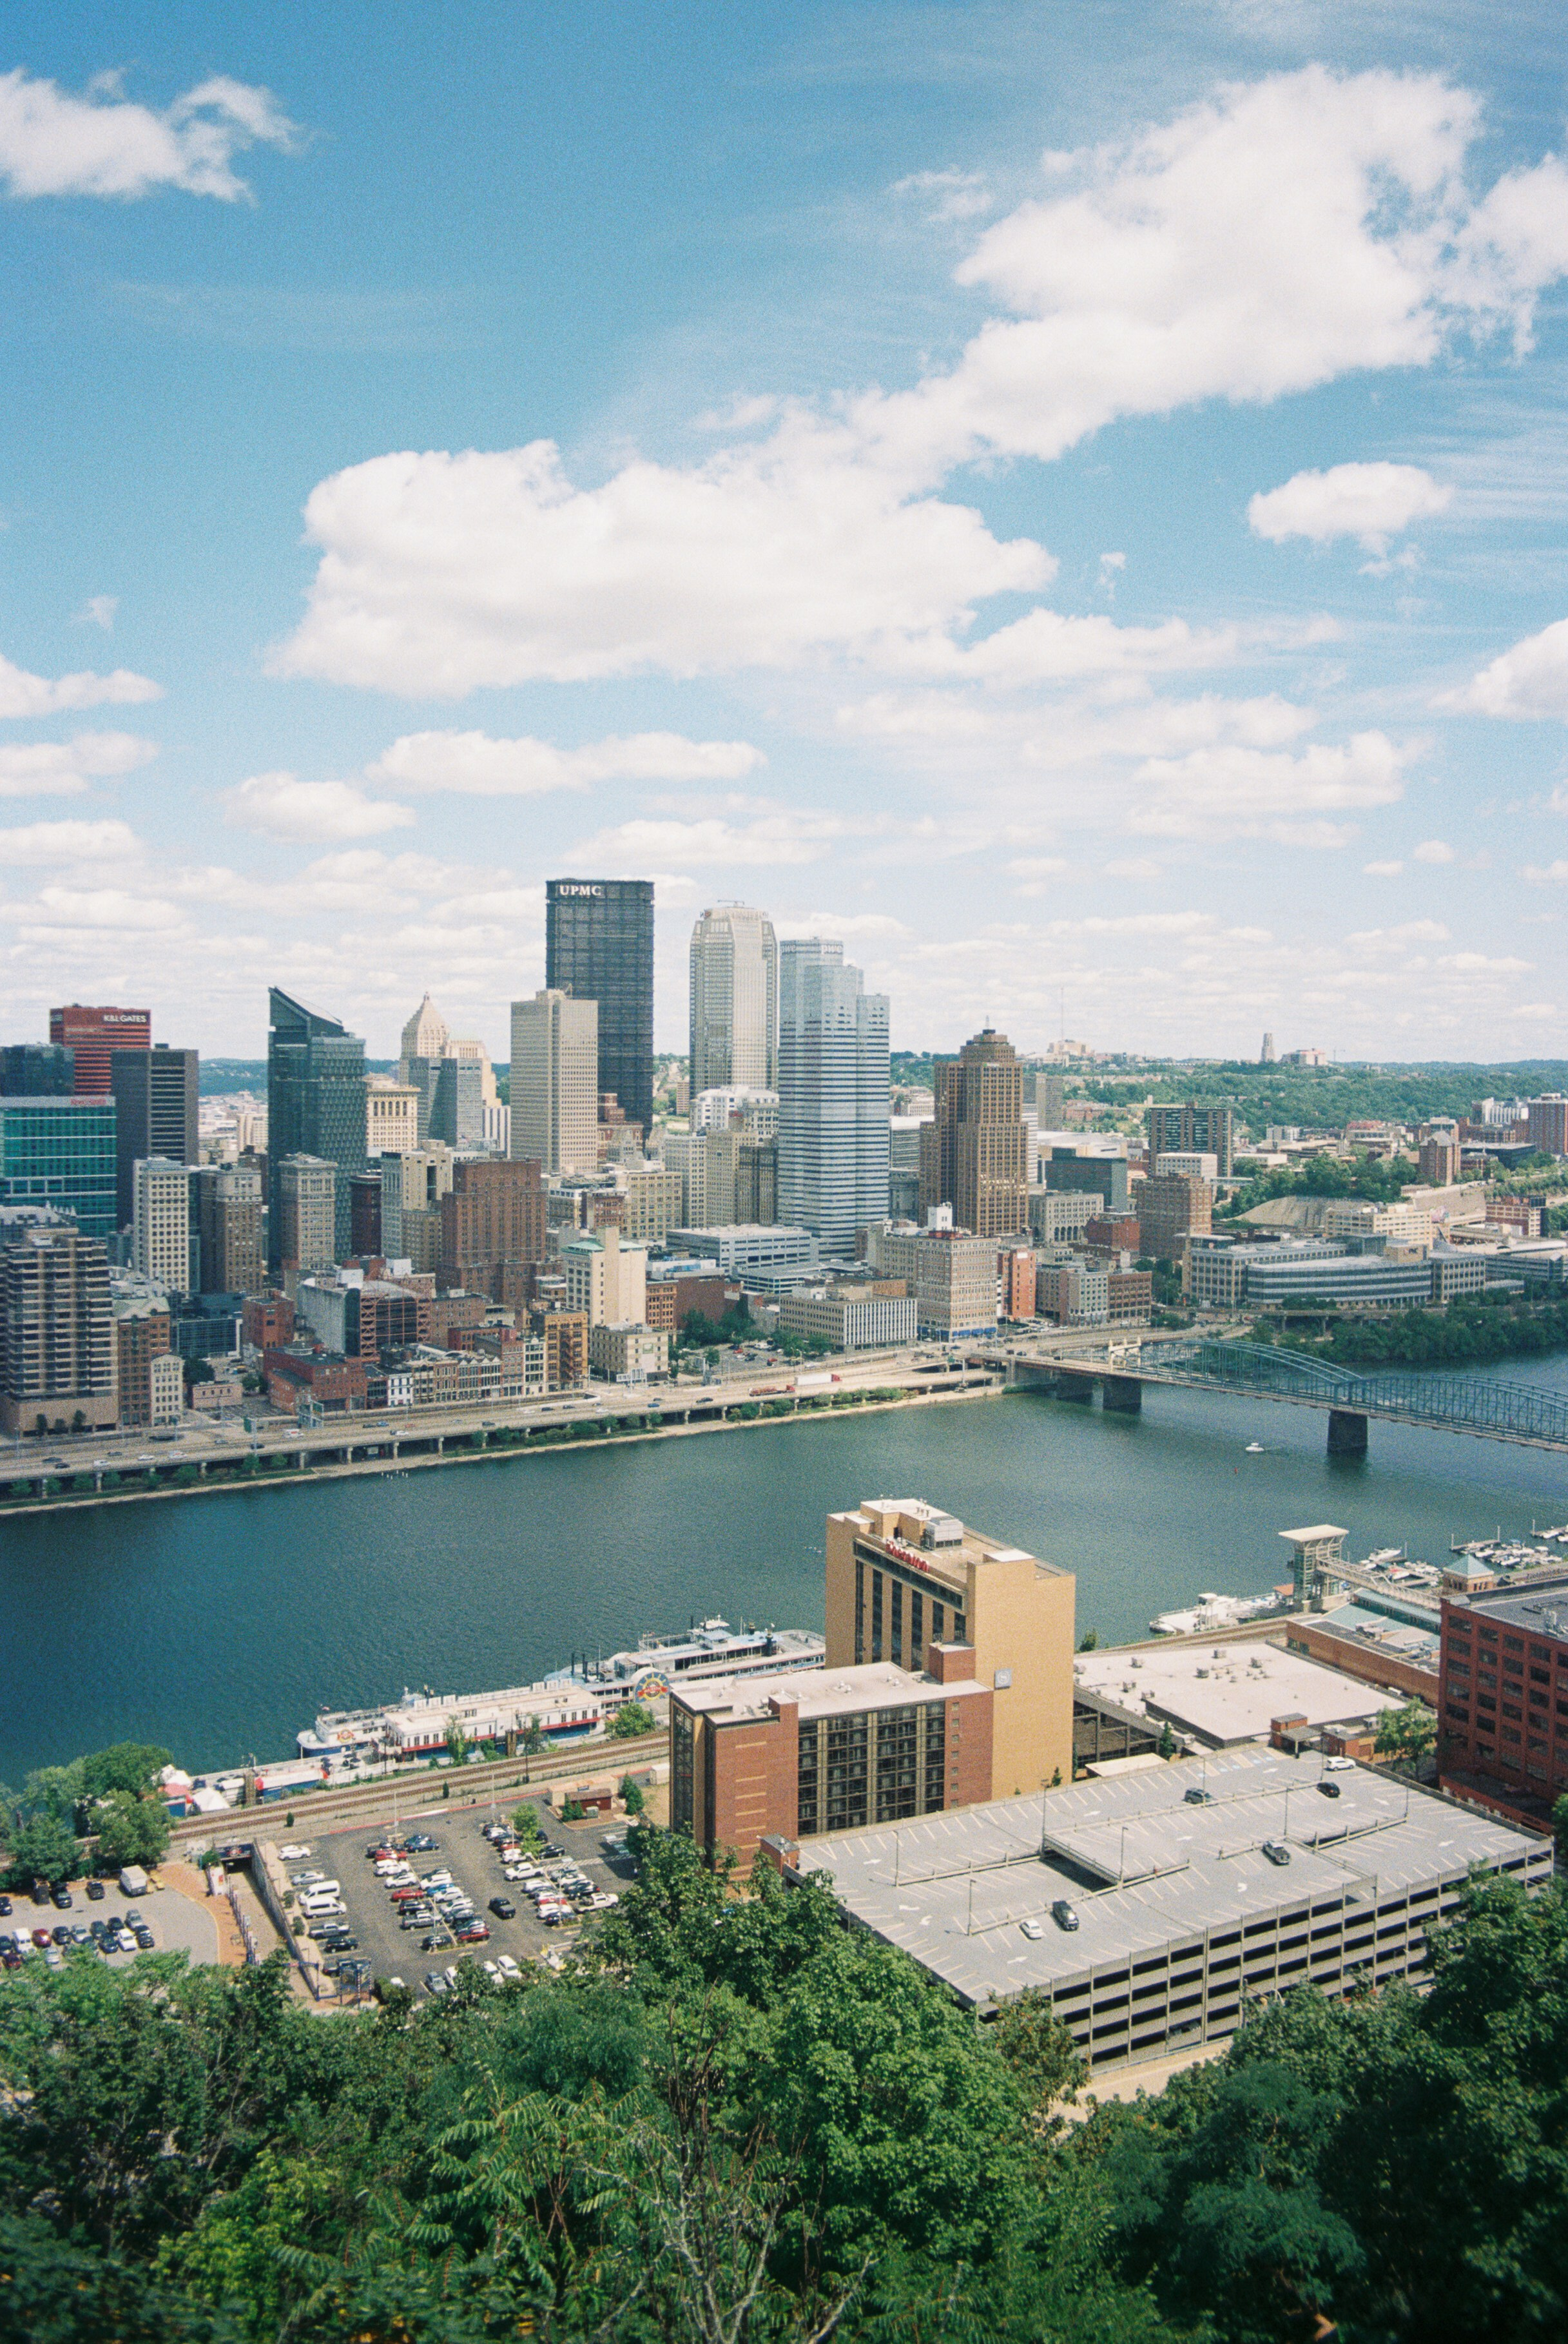
\includegraphics[scale=0.385]{./Images/banner.jpg}}} % Image background
\centering
\vspace*{5cm}
\par\normalfont\fontsize{35}{35}\sffamily\selectfont
\textbf{MAT389H1 Fall 2024}\\
{\LARGE Complex Analysis}\par % Book title
\vspace*{1cm}
{\Huge Nasrudeen Oladimeji}\par % Author name
\endgroup

%----------------------------------------------------------------------------------------
%	COPYRIGHT PAGE
%----------------------------------------------------------------------------------------

\newpage
~\vfill
\thispagestyle{empty}

%\noindent Copyright \copyright\ 2014 Andrea Hidalgo\\ % Copyright notice

\noindent\textsc{University of Toronto}\\

\noindent \textsc{github.com/Nasr-905}\\ % URL

\noindent Professor: Tristan Collins (tristan.collins@utoronto.ca)\\ % License information

\noindent \textit{First release, September 2024} % Printing/edition date

%----------------------------------------------------------------------------------------
%	TABLE OF CONTENTS
%----------------------------------------------------------------------------------------

\chapterimage{./Images/head1.jpg} % Table of contents heading image

\pagestyle{empty} % No headers

\tableofcontents % Print the table of contents itself

%\cleardoublepage % Forces the first chapter to start on an odd page so it's on the right

\pagestyle{fancy} % Print headers again

\chapterimage{./Images/head2.jpg} % Chapter heading image
\chapter{Complex Numbers}
\section{Introduction}
\begin{definition}
    [Complex Numbers]
    $z$ is a complex number iff $z = a + bi$ where $a, b \in \mathbb{R}$ and $i^2 = -1$. \\
    The set of complex numbers is denoted by $\mathbb{C}$.
\end{definition}
\begin{definition}
    [Real and Imaginary Parts]
    If $z = a + bi$, then $\Re(z) = a \in \mathbb{R}$ and $\Im(z) = b \in \mathbb{R}$. where $\Re(z)$ is the real part of $z$ and $\Im(z)$ is the imaginary part of $z$.
\end{definition}

\begin{definition}
    [Modulus]
    If $z = a + bi$, then $|z| = \sqrt{a^2 + b^2}$. $|z|$ is the modulus of $z$.
\end{definition}

\begin{definition}
    [Conjugate]
    If $z = a + bi$, then $\overline{z} = a - bi$. $\overline{z}$ is the conjugate of $z$.
\end{definition}
\section{Operations}
\begin{definition}
    [Addition and Subtraction]
    If $z_1 = a_1 + b_1i$ and $z_2 = a_2 + b_2i$, then $z_1 + z_2 = (a_1 + a_2) + (b_1 + b_2)i$. \\
    Similarly $z_1 - z_2 = (a_1 - a_2) + (b_1 - b_2)i$.
\end{definition}

\begin{definition}
    [Multiplication]
    If $z_1 = a_1 + b_1i$ and $z_2 = a_2 + b_2i$, then $z_1 \cdot z_2 = (a_1a_2 - b_1b_2) + (a_1b_2 + a_2b_1)i$. \\
    \textit{    Note that $|z_1 \cdot z_2| = |z_1| \cdot |z_2|$.}
\end{definition}

\begin{definition}
    [Inversion]
    If $z = a + bi$, then $z^{-1} = \frac{\overline{z}}{|z|^2}= \frac{a}{a^2 + b^2} - \frac{b}{a^2 + b^2}i$.
\end{definition}
\begin{proof}
    Let's multiply by 1 in the form of the conjugate of $z$:
    \begin{align*}
        \frac{1}{z} = \frac{1}{z}\times \frac{\overline{z}}{\overline{z}} = \frac{\overline{z}}{z\overline{z}} = \frac{a - bi}{(a + bi)(a - bi)} = \frac{a - bi}{a^2 + b^2} = \frac{a}{a^2 + b^2} - \frac{b}{a^2 + b^2}i
    \end{align*}
\end{proof}

\begin{definition}
    [Division]
    For $z, w \in \mathbb{C}$, $\frac{w}{z} = w \cdot z^{-1} = \frac{w\overline{z}}{|z|^2}$.
\end{definition}
\begin{table}[htbp]
    \centering
    \caption{Properties of the Complex Conjugate}
    \begin{tabular}{|c|c|}
        \hline
        \textbf{Property}        & \textbf{Description}                                                              \\
        \hline
        Conjugate of the Sum     & $\overline{z_1 + z_2} = \overline{z_1} + \overline{z_2}$                          \\
        \hline
        Conjugate Modulus        & $ z \cdot \overline{z}= |z|^2$                                                    \\
        \hline
        Conjugate of a Conjugate & $\overline{\overline{z}} = z$                                                     \\
        \hline
        Product of Conjugates    & $\overline{z_1 \cdot z_2} = \overline{z_1} \cdot \overline{z_2}$                  \\
        \hline
        Conjugate of a Quotient  & $\overline{\left(\frac{z_1}{z_2}\right)} = \frac{\overline{z_1}}{\overline{z_2}}$ \\
        \hline
        Real Part Conjugate      & $Re(z) = \frac{z + \overline{z}}{2}$                                              \\
        \hline
        Imaginary Part Conjugate & $Im(z) = \frac{z - \overline{z}}{2i}$                                             \\
        \hline
        Real Number Check        & $z = \overline{z} \iff z \in \mathbb{R}$                                          \\
        \hline
        Imaginary Number Check   & $z = -\overline{z} \iff z \in \mathbb{I}$                                         \\
        \hline
        Function Linearity       & If $\alpha = f(z)$ then $\overline{\alpha} = \overline{f(z)} = f(\overline{z})$   \\
        \hline
    \end{tabular}
\end{table}

\begin{table}[htbp]
    \centering
    \caption{Properties of the Modulus in Complex Numbers}
    \begin{tabular}{|c|c|}
        \hline
        \textbf{Property}         & \textbf{Description}                                                           \\
        \hline
        Positivity                & $|z| \geq 0$, with equality if and only if $z = 0$                             \\
        \hline
        Triangle Inequality       & $||z_1| - |z_2|| \leq |z_1 \pm z_2| \leq |z_1| + |z_2|$                        \\
        \hline
        Multiplicative Property   & $|z_1 \cdot z_2| = |z_1| \cdot |z_2|$                                          \\
        \hline
        Division Property         & $\left|\frac{z_1}{z_2}\right| = \frac{|z_1|}{|z_2|}$, for $z_2 \neq 0$         \\
        \hline
        Conjugate                 & $|z| = |\overline{z}|$                                                         \\
        \hline
        Component Property        & $-|z| \leq Re(z) \leq |z|$                                                     \\ & $-|z| \leq Im(z) \leq |z|$ \\
        \hline
        Cauchy-Schwarz Inequality & $|z_1w_1 + \cdots + z_nw_n|^2 \leq \sum_{j=1}^{n}|z_j|^2\sum_{j=1}^{n}|w_j|^2$ \\
        \hline
    \end{tabular}
\end{table}

\begin{proof}
    Proof of the Multiplicative Property of the Modulus:
    \begin{align*}
        |z_1 \cdot z_2|^2 & = (z_1 \cdot z_2) \cdot (\overline{z_1} \cdot \overline{z_2}) \\
                          & = z_1 \cdot \overline{z_1} \cdot z_2 \cdot \overline{z_2}     \\
                          & = |z_1|^2 \cdot |z_2|^2
    \end{align*}
\end{proof}
\section{Polar Representation}
A complex number are vectors in $\mathbb{R}^2$, as such, they can be represented by a magnitude and a direction. \\

\begin{definition}[Polar Form]
    \begin{align}
         & z = r(\cos(\theta) + i\sin(\theta)) \label{polar} \\
         & : r = |z| \in \mathbb{R}^+ \notag
        \label{polar form}
    \end{align}
\end{definition}

\begin{figure}[htbp]
    \centering
    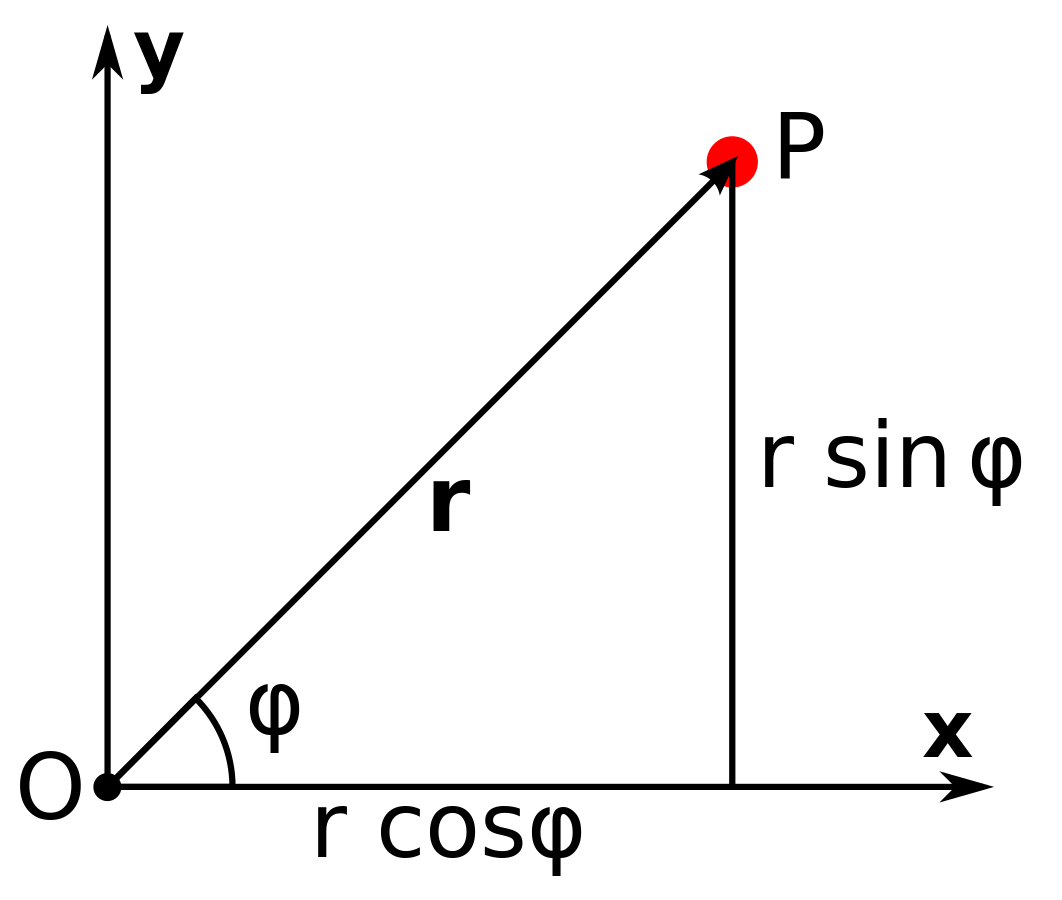
\includegraphics[scale = 0.2]{./LECTURE_1/Polar_coordinate_components.png}
    \caption{Polar Coordinate Components}
    \label{fig:polar}
\end{figure}

\begin{example}
    [Multiplying Complex Numbers in Polar Form]
    Let $z_1 = r_1(\cos(\theta_1) + i\sin(\theta_1))$ and $z_2 = r_2(\cos(\theta_2) + i\sin(\theta_2))$. Then:
    \begin{align}
        z_1 \cdot z_2 & = r_1r_2(\cos(\theta_1)\cos(\theta_2) - \sin(\theta_1)\sin(\theta_2) + i(\cos(\theta_1)\sin(\theta_2) + \sin(\theta_1)\cos(\theta_2))) \\
                      & = r_1r_2(\cos(\theta_1 + \theta_2) + i\sin(\theta_1 + \theta_2))
        \label{polar product}
    \end{align}
    Using the trig addition formula:
    \[\cos(\alpha + \beta) = \cos(\alpha)\cos(\beta) - \sin(\alpha)\sin(\beta)$ and $\sin(\alpha + \beta) = \cos(\alpha)\sin(\beta) + \sin(\alpha)\cos(\beta).\]
\end{example}

\begin{theorem}[De Moivre's Theorem]
    if $z = r(\cos(\theta) + i\sin(\theta))$
    \begin{align}
        z^n = r^n(\cos(\theta n) + i\sin(\theta n)) \label{Moivre}
    \end{align}
\end{theorem}

\begin{proof}
    \textit{The following proof will illustrative the steps to inductive reasoning}\\
    Case of $n = 1$: $z^n = r^n(\cos(\theta n) + i\sin(\theta n)) = z = r(\cos(\theta) + i\sin(\theta))$ \\
    This is true by definition. \\
    Assume that: \\
    $z^{n-1} = r^{n-1}(\cos(\theta (n-1)) + i\sin(\theta (n-1)))$ \\
    Then from Equation \eqref{polar product} we can verify: \\
    \begin{align}
        zz^{n-1} & = rr^{n-1}(\cos(\theta (n-1) + \theta) + i\sin(\theta (n-1) + \theta)) \notag \\
        z^{n}    & = r^{n}(\cos(\theta n) + i\sin(\theta n)) \notag
    \end{align}
\end{proof}

\begin{definition}
    [Argument]
    The argument of a complex number $z = r(\cos(\theta) + i\sin(\theta))$ is any angle, $\arg(z) = \theta$, such that $z = r(\cos(\theta) + i\sin(\theta))$.
\end{definition}

From Equation \eqref{polar}, we observe that $r$ is unique (because we constrained it to just positive values). $\theta$, however, is not unique.

\begin{definition}[Principle Orientation]
    We say $\theta$ is the principle orientation of $z$ if $\theta \in [-\pi, \pi)$ \\
    In this range, $\theta$ is unique.
\end{definition}

\begin{definition}
    [Vector Dot Product] The dot product of two vectors $a = (a_1, a_2)$ and $b = (b_1, b_2)$ is given by:
    \begin{align}
        a \cdot b  = \Re(a\overline{b})
        \label{dot product}
    \end{align}
    \begin{align}
        \cos \theta = \frac{a \cdot b}{|a||b|}
    \end{align}
\end{definition}

\begin{corollary}
    [Perpendicular Vectors]
    Complex variables $z$ and $w$ are perpendicular if $\Re(z\overline{w}) = 0$.
\end{corollary}

\begin{remark}
    [Complex Numbers to Solve Polynomial Equations]
    Over $\mathbb{C}$, every equation of the form $z^n = a$ has $n$ solutions.
\end{remark}
\begin{example}
    [Solving $z^n = -1$]
    Let $z = r(\cos(\theta) + i\sin(\theta))$. Then:
    \begin{align*}
        z^n               & = r^n(\cos(\theta n) + i\sin(\theta n)) = -1                                                               \\
        \implies r^n      & = 1 \text{ and } \cos(\theta n) + i\sin(\theta n) = -1                                                     \\
        \implies r        & = 1 \text{ and } \cos(\theta n) = -1 \text{ and } \sin(\theta n) = 0                                       \\
        \implies \theta n & = \pi + 2\pi k \text{ for } k \in \mathbb{Z}                                                               \\
        \implies \theta   & = \frac{\pi + 2\pi k}{n} \text{ for } k \in \mathbb{Z}                                                     \\
                          & \text{We can now find the principle solutions for } Z                                                      \\
                          & \therefore \theta_0 = \frac{\pi}{n}, \theta_1 = \frac{3\pi}{n}, \ldots, \theta_{n-1} = \frac{(2n-1)\pi}{n}
    \end{align*}
\end{example}
\begin{remark}
    Roots of Unity
    The solutions to $z^n = 1$ are called the $n$th roots of unity. Plotting these solutions splits the complex plane into $n$ equal parts.
    \begin{figure}
        \centering
        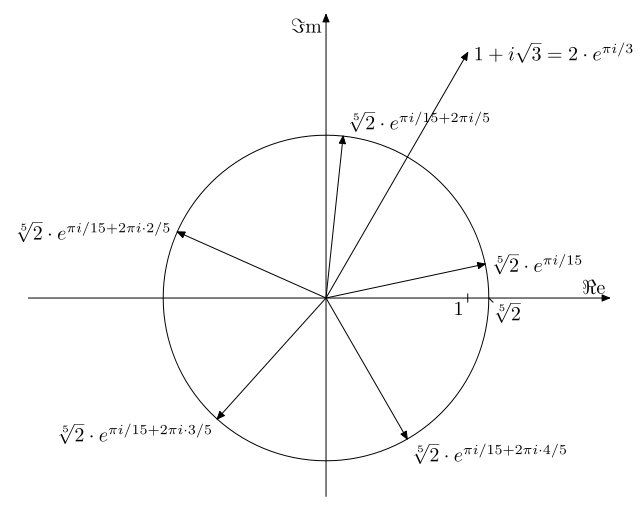
\includegraphics[scale = 0.2]{./LECTURE_1/Complex_fifth_roots.png}
        \caption{Complex Fifth Roots of Unity}
        \label{fig:roots}
    \end{figure}
\end{remark}
\section{Subsets of the Plane}
\begin{definition}
    [Open Disc]
    An open disc of radius $R$ centered at $z_0$ is the set of all $z$ such that $D_R(z_0) = \{z \in \mathbb{C} : |z - z_0| < R \subset \mathbb{C}\}$.
\end{definition}
\begin{definition}
    [Interior Point]
    A point $z_0$ is an interior point of a set $A \subset \mathbb{C}$ if there exists an open disc centered at $z_0$ that is contained in $A$.
    \[z_0 \text{is an interior point of $A$ if} \exists D_{>0}(z_0)\in A\]
\end{definition}

\begin{definition}
    [Open Set]
    A set $A \subset \mathbb{C}$ is open if every point in $A$ is an interior point. \\
    \textit{I.e. there are no 'hard lines' in the set.}
\end{definition}

\begin{example}
    [Open Disc]
    Show that the disc $D_R(z_0) = \{z \in \mathbb{C} : |z - z_0| < R\}$ is an open set.
    \begin{proof}
        Let $z_1 \in D$. Then $|z_1 - z_0| < R$. Let $r = R - |z_1 - z_0|$. Then $r > 0$. \\
        Let $z_2 \in D$ be any point in $D$, such that $|z_2 - z_1| < r$. Then:
        \begin{align*}
            |z_2 - z_0| & \leq |z_2 - z_1| + |z_1 - z_0| \\
                        & < r + R - r = R
        \end{align*}
        Therefore $z_2 \in D$ and $D$ is open.
    \end{proof}
\end{example}

\begin{definition}
    [Boundary ($\partial D$)]
    The boundary of a set $A$ is the set of all points $z$ such that every open disc centered at $z$ contains points in $A$ and points not in $A$. \\
    The boundary of $A$ is denoted by $\partial A$ and a boundary point $z$ is denoted by $z \in \partial A$.
    \[z_0 \text{is an boundary point of $A$ if} \exists z \in D_{R}(z_0) :z \notin A \forall R> 0\]
\end{definition}

\begin{definition}
    [Closed Set]
    A set $D$ is closed if it contains all its boundary points.
\end{definition}
\begin{remark}
    A set can be both open and closed ($\mathbb{C}, \emptyset$), open and not closed, closed and not open, or neither open nor closed.
\end{remark}
\begin{theorem}
    [Properties of Open and Closed Sets]
    \begin{enumerate}
        \item $D$ is open iff $\mathbb{C} \setminus D$ is closed.
        \item $D$ is closed iff $\mathbb{C} \setminus D$ is open.
        \item $D$ is open if and only if it contains none of its boundary points.
    \end{enumerate}
\end{theorem}

\chapter{Connectedness}
\section{Lecture 2: Connected Sets}
\begin{definition}
    [Connected Set]
    An \textit{open} set $D$ is connected if each pair of points $p, q \in D$ can be joined by a polygonal path lying entirely in $D$. That is:
    \[
        \exists P_2, P_3, \ldots, P_n \in D\quad  \text{ such that }\quad  pP_1, P_1P_2, \ldots, P_nq \in D\]
\end{definition}

\begin{remark}
    The set doesn't \textit{have} to be open, but it is easier to prove connectedness for open sets.
\end{remark}

\begin{figure}[H]
    \centering
    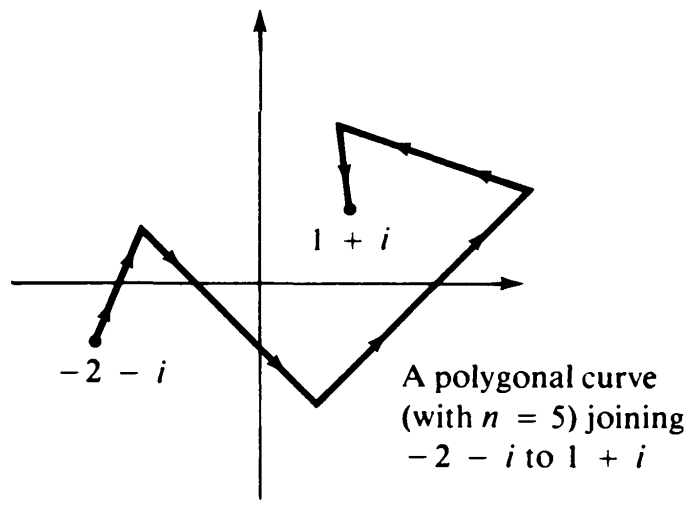
\includegraphics[scale=0.5]{LECTURE_2/poly.png}
    \caption{Polygonal Path}
    \label{fig:poly}
\end{figure}

\begin{definition}
    [Domain]
    A domain is a set that's
    \begin{itemize}
        \item Open
        \item Connected
        \item Not empty
    \end{itemize}
\end{definition}

\begin{definition}
    [Convex Set]
    A set $D$ is convex if for each pair of points $p, q \in D$, the line segment $pq$ lies entirely in $D$.
\end{definition}

\begin{figure}[H]
    \centering
    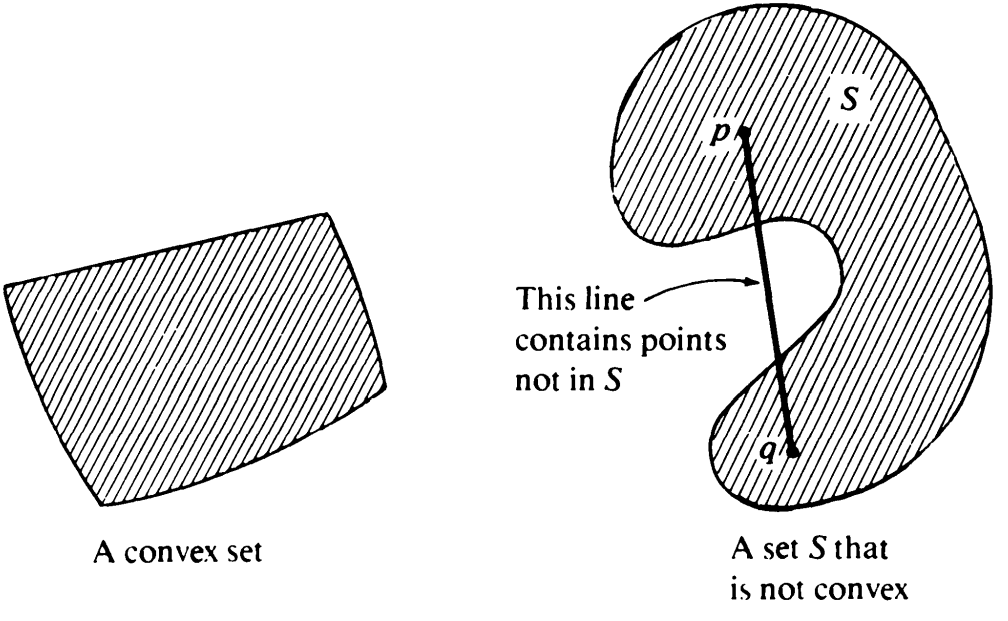
\includegraphics[scale=0.5]{LECTURE_2/convex.png}
    \caption{Convex Set}
    \label{fig:convex}
\end{figure}

\begin{theorem}
    [Convex $\implies$ Connected]
    If $D$ is a convex open set, then $D$ is connected.
\end{theorem}

\begin{definition}
    [Open Half-plane]
    A set $D$ is an open half-plane if it is of the form
    \[
        D = \{z \in \mathbb{C} : \Re\{az + b\} \geq 0\}
    \]
    \textit{Each open half-plane is convex and open}
\end{definition}

\begin{definition}
    [Closed Half-plane]
    A set $D$ is a closed half-plane if it is of the form
    \[
        D = \{z \in \mathbb{C} : \Re\{az + b\} > 0\}
    \]
    \textit{Each closed half-plane is convex and closed}
\end{definition}

\section{Point at Infinity}
\begin{definition}
    [Point at Infinity]
    A set is said to contain the point at infinity if it contains all points $z$ such that $|z| > R$ for some $R > 0$.
\end{definition}

\begin{example}
    No open Half-plane contains the point at infinity. Even though the set is unbounded, choosing $R$ near the boundary will always give a point outside the set.
\end{example}

\section{Functions and Limits}

\begin{definition}
    [Limit of a Sequence of Complex Numbers]
    \begin{align}
         & \lim_{n \to \infty} z_n = z \quad \text{or}\quad z_n \to z \iff \forall \epsilon > 0, \exists N \in \mathbb{N} \\
         & \text{such that} \quad n \geq N \implies |z_n - z| < \epsilon
    \end{align}
\end{definition}

\begin{corollary}
    [Parts of a Limit]
    If $z_n = x_n + iy_n$ and $z = x + iy$, then
    \[
        \lim_{n \to \infty} z_n = z \iff \lim_{n \to \infty} x_n = x \text{ and } \lim_{n \to \infty} y_n = y
    \]
\end{corollary}

\begin{theorem}
    [Subsequence]
    Suppose $\{z_n\}$ converges with limit $z$. Then every subsequence, $z_{m_n} = f(n)$ also converges to $z$. Where $ 1 \leq m_1 < m_2 < \ldots$
\end{theorem}

\begin{definition}
    [Limits of Functions]
    \begin{align}
         & \lim_{z \to z_0} f(z) = w \iff \forall \epsilon > 0, \exists \delta > 0 \\
         & \text{such that} 0 < |z - z_0| < \delta \implies |f(z) - w| < \epsilon
    \end{align}
\end{definition}

\section{Continuity}
\begin{definition}
    [Continuous Function]
    A function $f(z)$ is continuous at $z_0$ if
    \[
        \lim_{z \to z_0} f(z) = f(z_0)
    \]
\end{definition}

\begin{corollary}
    [Continuous at Infinity]
    A function $f(z)$ can be continuous at $\infty$ if $f(\infty) = \lim_{z\to \infty}f(z) = f(\infty)$. Note, $f(\infty)$ may equal $\infty$ \\
    \textit{This is equivalent to saying that $f(1/z)$ is continuous at $z = 0$}
\end{corollary}

\chapter{Series and Sequences}

\begin{definition}
    [infinite Series]
    Suppose we have a sequence:
    \begin{equation}
        z_1, z_2, z_3, \ldots
    \end{equation}
    We can define the partial sum of the sequence as:
    \begin{equation}
        S_n = z_1 + z_2 + z_3 + \ldots + z_n
    \end{equation}
    We say $\sum_{n=1}^{\infty} z_n$ converges and has a sum $S$ if the sequence of partial sums converges to $S$:
    \begin{equation}
        \lim_{n \to \infty} S_n = S
    \end{equation}
    If $\lim_{n \to \infty} S_n$ does not exist, we say the series diverges.
\end{definition}

\begin{corollary}
    [Real and Imaginary Parts of a Series]
    If $\sum_{n=1}^{\infty} z_n$ converges, then the real and imaginary parts of the series also converge.
    \begin{equation}
        \sum_{n=1}^{\infty} z_n = \sum_{n=1}^{\infty} \Re(z_n) + i \sum_{n=1}^{\infty} \Im(z_n)
    \end{equation}
\end{corollary}

\section{Tests for Convergence}
\begin{theorem}
    If $\sum_{n=1}^{\infty} z_n$ converges, then so does $\sum_{n=1}^{\infty} z_n$ and:
    \[
        \left| \sum_{n=1}^{\infty} z_n \right| \leq \sum_{n=1}^{\infty} |z_n|
    \]
\end{theorem}

\begin{proof}
    Say $z_n = x_n + i y_n$. Then:
    \begin{align}
         & \left| \sum_{n=1}^{\infty} x_n \right| & \leq \sum_{n=1}^{\infty}  \left| x_n \right| \leq \sum_{n=1}^{\infty}  \left| z_n \right| \\
         & \text{And}                                                                                                                         \\
         & \left| \sum_{n=1}^{\infty} y_n \right| & \leq \sum_{n=1}^{\infty}  \left| y_n \right| \leq \sum_{n=1}^{\infty}  \left| z_n \right|
    \end{align}
    So if $\sum_{n=1}^{\infty} x_n$ and $\sum_{n=1}^{\infty} y_n$ converge, then $\sum_{n=1}^{\infty} z_n$ converges.
\end{proof}

\begin{table}[htbp]
    \centering
    \begin{tabular}{| m{3cm} | m{7cm} | m{4cm} |}
        \hline
        \textbf{Test Name}         & \textbf{Description}                                                                                                                   & \textbf{Conditions for Use}                                         \\
        \hline
        Ratio Test                 & Uses the limit of the ratio of successive terms to determine convergence. \[ \lim_{n \to \infty} \left| \frac{a_{n+1}}{a_n} \right| \] & Applicable when terms are positive and the limit exists.            \\
        \hline
        Root Test                  & Uses the limit of the nth root of the terms to determine convergence. \[ \lim_{n \to \infty} \sqrt[n]{|a_n|} \]                        & Applicable when terms are positive and the limit exists.            \\
        \hline
        Integral Test              & Compares a series to an improper integral to determine convergence. \[ \int_{1}^{\infty} f(x) \, dx \]                                 & Applicable when terms are positive, continuous, and decreasing.     \\
        \hline
        Comparison Test            & Compares a series to a known convergent or divergent series.                                                                           & Applicable when terms are positive.                                 \\
        \hline
        Limit Comparison Test      & Compares the limit of the ratio of terms to a known series. \[ \lim_{n \to \infty} \frac{a_n}{b_n} \]                                  & Applicable when terms are positive and the limit exists.            \\
        \hline
        Alternating Series Test    & Determines convergence for series with alternating positive and negative terms.                                                        & Applicable when terms decrease in absolute value and approach zero. \\
        \hline
        p-Series Test              & Determines convergence based on the exponent in a series of the form \[ \sum \frac{1}{n^p} \]                                          & Applicable for series of the form \(\frac{1}{n^p}\).                \\
        \hline
        Geometric Series Test      & Determines convergence for geometric series. \[ \sum ar^n \]                                                                           & Applicable for series of the form \(ar^n\).                         \\
        \hline
        D'Alembert's Ratio Test    & Similar to the Ratio Test, but specifically for series with factorial terms.                                                           & Applicable when terms involve factorials.                           \\
        \hline
        Cauchy's Condensation Test & Determines convergence by condensing the series. \[ \sum a_n \sim \sum 2^n a_{2^n} \]                                                  & Applicable for series with positive, decreasing terms.              \\
        \hline
    \end{tabular}
    \caption{Common Tests for Convergence of Series}
    \label{table:convergence_tests}
\end{table}


\begin{example}
    \begin{align}
        \sum_{j=1}^{\infty} j \left( \frac{1 + 2i}{3} \right)^j &
    \end{align}
    We can use the ratio test to determine convergence:
    \begin{align}
        \sum_{j=1}^{\infty} \left| z_j \right|                 & = \sum_{j=1}^{\infty} j \left| \frac{1 + 2i}{3} \right|^j                                 \\
                                                               & = \sum_{j=1}^{\infty} j \left( \frac{\sqrt{5}}{3} \right)^j                               \\
        \lim_{j \to \infty} \left| \frac{z_{j+1}}{z_j} \right| & = \lim_{j \to \infty} \frac{(j+1)({\frac{\sqrt{5}}{3}})^{j + 1}}{j(\frac{\sqrt{5}}{3})^j} \\
                                                               & = \lim_{j \to \infty} \frac{j+1}{j} \left( \frac{\sqrt{5}}{3} \right)                     \\
                                                               & = \frac{5}{3} < 1
                                                               & \therefore \text{The series converges}
    \end{align}
\end{example}

\section{The Exponential Function}
\subsection*{Approach 1}
\begin{definition}
    [Exponential Function]
    If $z = x + iy$, then the exponential function is defined as:
    \begin{equation}
        e^z = e^x \left( \cos(y) + i \sin(y) \right)
    \end{equation}
\end{definition}

\begin{remark}
    [Euler's Formula]
    \begin{align}
        e^{i\theta} & \triangleq \cos(\theta) + i \sin(\theta) \\
    \end{align}
\end{remark}

\subsection*{Properties of the complex Exponential Function}
\begin{table}[htbp]
    \centering
    \begin{tabular}{| m{2.5cm} | m{11.5cm} |}
        \hline
        \textbf{Property} & \textbf{Description}                                                                                                                      \\
        \hline
        Periodicity       & The complex exponential function is periodic with period \( 2\pi i \), \[ e^{z + 2\pi i} = e^z \].                                        \\
        \hline
        Multiplication    & The exponential function satisfies \[ e^{z_1 + z_2} = e^{z_1} e^{z_2} \] for any complex numbers \( z_1 \) and \( z_2 \).                 \\
        \hline
        Derivative        & The derivative of the exponential function is \[ \frac{d}{dz} e^z = e^z \].                                                               \\
        \hline
        Inverse           & The inverse of the exponential function is the complex logarithm, \[ \log z \], such that \[ e^{\log z} = z \] for \( z \neq 0 \).        \\
        \hline
        Magnitude         & The magnitude of the exponential function is \[ |e^z| = e^{\Re(z)} \], where \( \Re(z) \) denotes the real part of \( z \).               \\
        \hline
        Argument          & The argument of the exponential function is \[ \arg(e^z) = \Im(z) \mod 2\pi \], where \( \Im(z) \) denotes the imaginary part of \( z \). \\
        \hline
        Conjugate         & The conjugate of the exponential function is \[ \overline{e^z} = e^{\overline{z}} \].                                                     \\
        \hline
    \end{tabular}
    \caption{Properties of the Complex Exponential Function}
    \label{table:complex_exponential_properties}
\end{table}

\subsection*{Approach 2: Taylor Series}

\begin{definition}
    [The Exponential Function]
    The exponential function can be defined as:
    \begin{equation}
        e^z = \sum_{n=0}^{\infty} \frac{z^n}{n!} \qquad \text{for all } z \in \mathbb{C}
    \end{equation}
\end{definition}

\begin{claim}
    [The Taylor Series for the Exponential Function Converges]
    $\sum_{n=0}^{\infty} \frac{z^n}{n!}$ converges for all $z \in \mathbb{C}$.
\end{claim}
\begin{proof}
    HOMEWORK
\end{proof}

\begin{problem}
For $\theta \in \mathbb{R}$
\[
    e^{i\theta} = \sum_{n=0}^{\infty} \frac{(i\theta)^n}{n!} = \cos(\theta) + i \sin(\theta)
\]
\end{problem}

\section{Approach 3: Differential Equations}
\begin{definition}
    [Differential Equation for the Exponential Function]
    The exponential function satisfies the differential equation:
    \begin{equation}
        f(z) = \begin{cases}
            \frac{df}{dz} = f & \text{for all } z \in \mathbb{C} \\
            f(0) = 1
        \end{cases}
    \end{equation}
\end{definition}

\section{The Logarithm Function}
\begin{definition}
    [Logarithm Function]
    The logarithm function is defined as the inverse of the exponential function:
    \begin{equation}
        \log z = \log |z| + i \theta
    \end{equation}
\end{definition}
\begin{remark}
    There will be many solutions to the logarithm function, as the argument is only defined modulo \(2\pi\).
    \[
        \log z = \log |z| + i \left( \arg(z) + 2\pi n \right) \qquad \text{for } n \in \mathbb{Z}
    \]
\end{remark}

\begin{definition}
    [Principal Logarithm]
    The principal branch logarithm is defined as:
    \[
        \text{Log}(z) = \log |z| + i \arg(z) \qquad \text{for } -\pi < \arg(z) \leq \pi
    \]
    \textit{Note: We use a capital L to denote the principal logarithm.}
\end{definition}

\begin{definition}
    [Fixed $\theta_0$ Logarithm Function]
    We can fix the argument of the logarithm function by setting \(\theta_0\) and letting $D = \{ te^{i\theta_0} | t > 0, t \in \mathbb{R} \}$.\\
    We define:
    \[
        \widetilde{\log}_{\theta_0} z = \log |z| + i \left( \widetilde{\arg}(z) + \theta_0 \right) \qquad \text{for } z \in D, \arg(z) \in [\theta_0, \theta_0 + 2\pi)
    \]
\end{definition}

\begin{example}
    [Find the Values of $(-1)^i$]
    \begin{align}
        (-1)^i   & = e^{i \log(-1)}                         \\
                 & = e^{i (2n + 1)\pi i}                    \\
                 & = e^{-2n\pi}                             \\
        \log(-1) & = -(2n + 1)\pi i \qquad n \in \mathbb{Z} \\
        (-1)^i   & = e^{2n + 1}\pi
    \end{align}
\end{example}

\section{The Trigonometric Functions}
\begin{definition}
    [Trigonometric Functions]
    For $z \in mathbb{C}$ trigonometric functions are defined as:
    \begin{align}
        \Re{e^{iz}} & = \cos(z)  = \frac{e^{iz} + e^{-iz}}{2}  \\
        \Im{e^{iz}} & = \sin(z)  = \frac{e^{iz} - e^{-iz}}{2i} \\
        \tan(z)     & = \frac{\sin(z)}{\cos(z)}                \\
    \end{align}
\end{definition}

\begin{lemma}
    \begin{align}
        \begin{cases}
            \cos(z + \alpha) = \cos(z) \\
            \sin(z + \alpha) = \sin(z)
        \end{cases}
    \end{align}
    iff $\alpha = 2\pi n$ for $n \in \mathbb{Z}$.
\end{lemma}

\begin{proof}
    \begin{align}
        e^{i(z + \alpha)} & = e^{iz} e^{i\alpha}                                   \\
                          & = e^{iz} \left( \cos(\alpha) + i \sin(\alpha) \right)  \\
                          & = e^{iz} \left( \cos(2\pi n) + i \sin(2 \pi n) \right) \\
                          & = e^{iz}
    \end{align}
\end{proof}

% \chapter{Line Integrals: Green's Continuous  Map}
\begin{theorem}
    [Parametrized Curves]
    $$ \gamma (t) = x(t) + iy(t) \quad a \leq t \leq b $$
    $\gamma [a,b] \to \mathbb{C}$ is the image of $\gamma$.
\end{theorem}

\begin{definition}
    [Simple Curve]
    A curve $\gamma$ is \textbf{simple} if $\gamma(t_1) = \gamma(t_2) \implies t_1 = t_2$ for $t_1, t_2 \neq a, b$.
\end{definition}
\begin{definition}
    [Closed Curve]
    A curve $\gamma$ is \textbf{closed} if $\gamma(a) = \gamma(b)$. So if the end point meets the starting point.
\end{definition}

\begin{remark}
    We can \textit{ignore} the parametrization and talk about the curve $$Image(\gamma) \subset \mathbb{C}$$ as a subset of $\mathbb{C}$.
\end{remark}

\begin{definition}
    [$C^1$/Smooth Curve]
    A parametrized curve is $C^1$ if $\gamma'(t)$ if
    $$\gamma '(t) = x'(t) + iy'(t)$$ exists $\forall t \in [a,b]$ and is continuous.
\end{definition}

\begin{remark}
    Here, $\gamma'(a), \gamma'(b)$ are the 1-sided derivatives.
\end{remark}

\begin{definition}
    [Piecewise $C^1$/Smooth Curve]
    $$\text{if } \exists a = t_0 < t_1 < \ldots < t_n = b \text{ such that } \gamma |_{[t_i, t_{i+1}]} \text{ is } C^1$$
\end{definition}

\section{Line Integrals}
\begin{definition}
    [Line Integral]
    if $g = u + iv, (u,v) \in \mathbb{R}^2$ is a complex-valued function and $\gamma$ is piecewise $C^1$, then the line integral of $g$ along $\gamma$ is
    $$\int_{\gamma} g(z) dz = \sum_{i=0}^{n-1}\int_{i}^{i+1} g(\gamma(t)) \gamma'(t) dt$$
    Where
    \begin{align*}
        g(\gamma(t)) \gamma'(t) & = ux' - vy' + ivx' + iuy'                        \\
                                & = (u(\gamma(t)) + iv(\gamma(t)))(x'(t) + iy'(t)) \\
    \end{align*}
    is complex multiplication
\end{definition}

\begin{theorem}
    [Length of a Curve]
    If $\gamma$ is a piecewise $C^1$ curve, then the length of $\gamma$ is
    $$\text{Length}(\gamma) = \sum_{i = 0}^{n-1}\int_{t_i}^{t_{i + 1}} |\gamma'(t)| dt$$
    So we have
    $$ |\int_{\gamma}g |\leq \max_{z \in \gamma}|g(z)| \cdot \text{Length}(\gamma) $$
\end{theorem}

\begin{theorem}
    [Green's Theorem]
    Say $ \Omega \subset \mathbb{C} $ such that $\partial \Omega$ is a finite collection of piecewise $C^1$ closed simple curves. If $g = u + iv$ is $C^1$ on $\Omega$, then
    % $$\int_{\partial \Omega} g = \int_{\Omega} \left( \frac{\partial v}{\partial x} - \frac{\partial u}{\partial y} \right) dxdy$$
    % Where $\partial \Omega$ is the boundary of $\Omega$.

    if $ = p + iq$ is differentiable in $\Omega$, then ($\Re{p, q}$ have $1^{st}$ order derivatives). Then
    $$\int_{\partial \Omega} f = i \int_{\Omega} \left( \frac{\partial f}{\partial x} - \frac{\partial f}{\partial y} \right) dxdy$$
    Where $\partial \Omega$ is the boundary of $\Omega$.
\end{theorem}

\begin{corollary}
    If $dz = dx + idy$, then
    \begin{align*}
        \Re(fdz) & = \Re(f)dx - \Im(f)dy \\
                 & = pdx - qdy           \\
        \Re{(i \left(\frac{\partial f}{\partial x} + \frac{i \partial f}{\partial y}\right))} = - \frac{\partial q}{\partial x} - \frac{\partial p}{\partial y}
    \end{align*}
    So
    \begin{align*}
        \int_{\partial \Omega} pdx + qdy = \left(
        \int_{\Omega} \left( \frac{\partial q}{\partial x} + \frac{\partial p}{\partial y} \right) dxdy
        \right)
    \end{align*}
\end{corollary}

\begin{remark}
    Orient $\partial \Omega$ always on the left (in the counter-clockwise direction outsides, conterclockwise insides) as we walk along $\partial \Omega$ (say $\partial \Omega$ is positively oriented).
\end{remark}

\begin{example}
    [Very Important Example]
    Let $\gamma$ be a simple, closed piecewise $C^1$ curve. such that $\gamma = \partial \Omega$ for some $\Omega \subset \mathbb{C}$. Then for $ p \notin \Omega$,
    $$ \frac{1}{2\pi i} \int_{\gamma} \frac{dz}{z - p} = \begin{cases}
            1 & \text{if } p \in \Omega    \\
            0 & \text{if } p \notin \Omega
        \end{cases} $$
    \begin{proof}
        1) Assume $p$ not in $\Omega$, then $\frac{1}{z - p}$ is differentiable in $\Omega$ and $\partial \Omega$ is a simple closed curve. So by Green's Theorem,
        $$ \int_{\partial \Omega} \frac{dz}{z - p} = i \int_{\Omega} \left( \frac{\partial}{\partial x} \frac{1}{z - p} - i\frac{\partial}{\partial y} \frac{1}{z - p} \right) dxdy = 0 $$
    \end{proof}
    Let $D_{\epsilon}(p)$ be the disk of radius $\epsilon$ centered at $p$, essentially, we want to remove the point stopping us from applying Green's Theorem.
    $$ \Omega_{\epsilon} = \Omega \setminus D_{\epsilon}(p) $$
    If $\epsilon$ is sufficiently small, $\Omega_{\epsilon}$ is still a domain. So by Green's Theorem,
    \begin{align*} \int_{\partial \Omega_{\epsilon}} \frac{dz}{z - p}                                         & = 0                                                                    \\
               \int_{\partial \Omega} \frac{dz}{z - p} - \int_{\partial D_{\epsilon}(p)} \frac{dz}{z - p} & = 0                                                                    \\
               \int_{\partial \Omega} \frac{dz}{z - p}                                                    & = \int_{\partial D_{\epsilon}(p)} \frac{dz}{z - p}                     \\
               \rightarrow \partial D_{\epsilon}                                                          & = p + \epsilon e^{it} \quad 0 \leq t \leq 2\pi                         \\
               \int_{\partial D_{\epsilon}(p)} \frac{dz}{z - p}                                           & = \int_{0}^{2\pi} \frac{i\epsilon e^{it}}{\epsilon e^{it}} dt = 2\pi i \\
               \int_{\partial \Omega} \frac{dz}{z - p}                                                    & = 2\pi i
    \end{align*}
\end{example}


% \chapter{Analytic Functions and the Cauchy-Riemann Equations}

\section{Analytic Functions}

\begin{definition}
    [Complex Differentiability]
    A complex function $f(z): D \to \mathbb{C}$, where $D$ is a domain, is \textbf{complex differentiable} at $z_0 \in D$ if
    $$f'(z_0) = \lim_{z \to z_0} \frac{f(z) - f(z_0)}{z - z_0} \quad \text{exists}$$
    $$ = \lim_{h} \frac{f(z_0 + h) - f(z_0)}{h} \quad h \in \mathbb{C}$$
\end{definition}

\begin{definition}
    [Analytic]
    A function $f(z)$ is \textbf{analytic} on a domain $D$ if $f(z)$ is complex differentiable at every point in $D$.
\end{definition}

\begin{definition}
    [Entire]
    A function $f(z)$ is \textbf{entire} if $f(z)$ is analytic on $\mathbb{C}$.
\end{definition}

\begin{example}
    [Prove the Power Rule]
    $$f(z) = z^n \quad n \in \mathbb{Z}$$
    $f$ is entire and
    $$f'(z) = nz^{n-1}$$
\end{example}
\begin{proof}
    \begin{align*}
        \lim_{h \to 0} \frac{f(z + h) - f(z)}{h} & = \lim_{h \to 0} \frac{(z + h)^n - z^n}{h}                               \\
                                                 & = \lim_{h \to 0} \frac{\sum_{k=0}^{n} \binom{n}{k} z^{n-k} h^k - z^n}{h} \\
                                                 & = \lim_{h \to 0} \sum_{k=0}^{n} \binom{n}{k} z^{n-k} h^{k-1}             \\
                                                 & = \binom{n}{1} z^{n-1}                                                   \\
                                                 & = nz^{n-1}                                                               \\
    \end{align*}
\end{proof}

\begin{example}
    Prove that $f(z) = \overline{z}$ is not complex differentiable at any point.
\end{example}
\begin{proof}
    In homework 2...
\end{proof}

\begin{table}[htbp]
    \centering
    \begin{tabular}{| m{5cm} | m{9cm} |}
        \hline
        \textbf{Property}       & \textbf{Description}                                                                                                                                                                               \\
        \hline
        Linearity               & The derivative of a sum is the sum of the derivatives: \[ (f + g)'(z) = f'(z) + g'(z) \] The derivative of a constant multiple is the constant multiple of the derivative: \[ (cf)'(z) = cf'(z) \] \\
        \hline
        Product Rule            & The derivative of a product is given by: \[ (fg)'(z) = f'(z)g(z) + f(z)g'(z) \]                                                                                                                    \\
        \hline
        Quotient Rule           & The derivative of a quotient is given by: \[ \left( \frac{f}{g} \right)'(z) = \frac{f'(z)g(z) - f(z)g'(z)}{g(z)^2} \]                                                                              \\
        \hline
        Chain Rule              & The derivative of a composition is given by: \[ (f \circ g)'(z) = f'(g(z))g'(z) \]                                                                                                                 \\
        \hline
        Exponential Function    & The derivative of the exponential function is: \[ \frac{d}{dz} e^z = e^z \]                                                                                                                        \\
        \hline
        Logarithmic Function    & The derivative of the logarithmic function is: \[ \frac{d}{dz} \log z = \frac{1}{z} \]                                                                                                             \\
        \hline
        Power Rule              & The derivative of a power function is: \[ \frac{d}{dz} z^n = nz^{n-1} \]                                                                                                                           \\
        \hline
        Trigonometric Functions & The derivatives of the trigonometric functions are: \[ \frac{d}{dz} \sin z = \cos z \] \[ \frac{d}{dz} \cos z = -\sin z \]                                                                         \\
        \hline
        Hyperbolic Functions    & The derivatives of the hyperbolic functions are: \[ \frac{d}{dz} \sinh z = \cosh z \] \[ \frac{d}{dz} \cosh z = \sinh z \]                                                                         \\
        \hline
    \end{tabular}
    \caption{Properties of Complex Derivatives}
    \label{table:complex_derivative_properties}
\end{table}

\begin{example}
    [Prove the Derivative of the Exponential Function]
    $$f(z) = e^z$$
\end{example}

\begin{proof}
    \begin{align*}
        \lim_{h \to 0} \frac{e^{z + h} - e^z}{h} & = \lim_{h \to 0} \frac{e^z e^h - e^z}{h}                          \\
                                                 & = e^z \lim_{h \to 0} \frac{e^h - 1}{h}                            \\
                                                 & = e^z \lim_{h \to 0} \frac{1 + h + \frac{h^2}{2} + \cdots - 1}{h} \\
                                                 & = e^z \lim_{h \to 0} 1 + \frac{h}{2} + \cdots                     \\
    \end{align*}
\end{proof}

\section{Cauchy-Riemann Equations}
\begin{lemma}
    [$h$ can approach from any direction]
    If $f(z)$ is differentiable then $$\exists\lim_{h \to 0} \frac{f(z + h) - f(z)}{h} = f(z) \in \mathbb{C}$$
    And yield the same result for any $h \in \mathbb{C}$.
\end{lemma}


\begin{theorem}
    [Cauchy-Riemann Equations]
    If $f(z) = u(x,y) + iv(x,y)$ is differentiable at $z = x + iy$, then
    $$\frac{\partial u}{\partial x} = \frac{\partial v}{\partial y} \quad \text{and} \quad \frac{\partial u}{\partial y} = -\frac{\partial v}{\partial x}$$
\end{theorem}


\begin{proof}
    We compute $h$ in two ways:
    \begin{align*}
        h_1 & = is \quad s \in \mathbb{R} \\
        h_2 & = s \in \mathbb{R}
    \end{align*}
    \begin{align*}
          & \lim_{h\to 0}\frac{f(z + is) - f(z)}{is}                                       \\
        = & lim_{h\to 0}\frac{u(x, y + s) + iv(x, y + s) - u(x, y) - iv(x, y)}{is}         \\
        = & lim_{h\to 0}\frac{u(x, y + s) - u(x, y)}{is} + \frac{v(x, y + s) - v(x, y)}{s} \\
        = & \frac{1}{i}(\frac{\partial u}{\partial y} + \frac{\partial v}{\partial y})
    \end{align*}

    \begin{align*}
          & \lim_{h\to 0}\frac{f(z + s) - f(z)}{s}                                         \\
        = & lim_{h\to 0}\frac{u(x + s, y) + iv(x + s, y) - u(x, y) - iv(x, y)}{s}          \\
        = & lim_{h\to 0}\frac{u(x + s, y) - u(x, y)}{s} + i\frac{v(x + s, y) - v(x, y)}{s} \\
        = & \frac{\partial u}{\partial x} + i\frac{\partial v}{\partial x}
    \end{align*}

    So
    \begin{align*}
        \frac{\partial u}{\partial x} + i\frac{\partial v}{\partial x} & = \frac{1}{i}(\frac{\partial u}{\partial y} + \frac{\partial v}{\partial y}) \\
        \frac{\partial u}{\partial x} - i\frac{\partial u}{\partial y} & = \frac{\partial v}{\partial y}                                              \\
        \frac{\partial u}{\partial x}                                  & = \frac{\partial v}{\partial y}                                              \\
        \frac{\partial u}{\partial y}                                  & = -\frac{\partial v}{\partial x}                                             \\
    \end{align*}


\end{proof}

\begin{theorem}
    [Harmonic Functions]
    If $f(z) = u(x,y) + iv(x,y)$ is complex differentiable, then
    $$ \Delta u  = \Delta v = 0$$
    And $u, v$ are \textbf{harmonic functions} and satisfy Cauchy-Riemann equations. Thus they are \textbf{harmonic conjugates}.
    Where $\Delta = \frac{\partial^2}{\partial x^2} + \frac{\partial^2}{\partial y^2}$ is the Laplacian operator.
\end{theorem}

\begin{corollary}
    If a function $f(z)$ is once complex differentiable, then it is infinitely differentiable and analytic.
\end{corollary}

\begin{proof}
    Cauchy-Riemann equations give us the partial derivatives of $u, v$.
    $$
        \begin{cases}
            \frac{\partial u}{\partial x} = \frac{\partial v}{\partial y} \\
            \frac{\partial u}{\partial y} = -\frac{\partial v}{\partial x}
        \end{cases}$$
    \begin{align*}                                                                                                                                                                                                                      \\
        \text{Take} \quad \frac{\partial}{\partial x}(1) \quad \frac{\partial^2 u}{\partial x^2} & = \frac{\partial}{\partial x} \frac{\partial u}{\partial x} = \frac{\partial}{\partial x} \frac{\partial v}{\partial y} = \frac{\partial}{\partial y} \frac{\partial v}{\partial x} = \frac{\partial}{\partial y} \frac{\partial u}{\partial y} = \frac{\partial^2 u}{\partial y^2} \\
        \text{Take} \quad \frac{\partial}{\partial y}(2) \quad \frac{\partial^2 u}{\partial y^2} & = -\frac{\partial}{\partial y} \frac{\partial v}{\partial x} = -\frac{\partial}{\partial x} \frac{\partial v}{\partial y} = -\frac{\partial}{\partial x} \frac{\partial u}{\partial y} = -\frac{\partial^2 u}{\partial x^2}                                                         \\
                                                                                                 & \Delta u = 0
    \end{align*}
\end{proof}

\begin{theorem}
    Let $f = u + iv$ and assume $u, v, \frac{\partial u}{\partial x}, \frac{\partial u}{\partial y}, \frac{\partial v}{\partial x}, \frac{\partial v}{\partial y}$ are defined and continuous on a disc around $z_0$. If $u, v$ satisfy the Cauchy-Riemann equations at $z_0$, then $f$ is complex differentiable at $z_0$.
    $$\frac{\partial f}{\partial z} = \frac{\partial u}{\partial x} + i\frac{\partial v}{\partial x}$$
\end{theorem}

\begin{proof}
    Using the taylor expansion of $f(z)$
    \begin{align*}
        \lim_{h \to 0} \frac{f(z_0 + h) - f(z_0)}{h} & = \lim_{h \to 0} \frac{u(x_0 + h, y_0) + iv(x_0 + h, y_0) - u(x_0, y_0) - iv(x_0, y_0)}{h}          \\
                                                     & = \lim_{h \to 0} \frac{u(x_0 + h, y_0) - u(x_0, y_0)}{h} + i\frac{v(x_0 + h, y_0) - v(x_0, y_0)}{h} \\
                                                     & = \frac{\partial u}{\partial x} + i\frac{\partial v}{\partial x}
    \end{align*}
\end{proof}


\begin{example}
    [Prove the Derivative of the Logarithmic Function]
    Let $D \in \mathbb{C}$ be a domain o which there is a single-valued branch of $\log z$.
\end{example}

\begin{proof}
    When $\arctan(y/x) \in (\theta_0, \theta + \pi]$ and $\arctan(y/x)$ is not in $D$.
    $$u = \frac{1}{2} \log(x^2 + y^2) \quad v = \arctan(y/x)$$
    Then
    \begin{align}
        \frac{\partial u}{\partial x}            & = \frac{1}{2(x^2+ y^2)} \cdot 2x = \frac{x}{x^2 + y^2} \\
        \frac{\partial v}{\partial y}            & = \frac{1}{1 + \frac{y}{x}^2} \times \frac{1}{x}       \\
                                                 & = \frac{x}{x^2 + y^2}                                  \\
        \therefore \frac{\partial u}{\partial x} & = \frac{\partial v}{\partial y}
    \end{align}
    INCOMPLETE
\end{proof}

% \chapter{Lecture 6: Power Series}

\section{Introduction}
\begin{definition}
    [Power Series]
    A power series in $z$ is a n infinite series of the form:
    $$\sum_{n=0}^{\infty} a_n (z-z_0)^n$$
    where $a_n$ are complex numbers, $z$ is a complex variable, and $z_0 \in \mathbb{C}$ is the centre.
\end{definition}

\begin{theorem}
    [Absolute Convergence of Power Series]
    Suppose $\exists z_1 \neq z_0 | \sum_{n=0}^{\infty} a_n (z_1-z_0)^n$ converges. Then for each $z \in \mathbb{C} : |z-z_0| < |z_1 - z_0|$, the series $\sum_{n=0}^{\infty} a_n (z-z_0)^n$ converges \textbf{absolutely}.
\end{theorem}

\begin{proof}
    Since $\sum_{n=0}^{\infty} a_n (z_1-z_0)^n$ converges, we know:
    \begin{equation}\lim_{n \to \infty} a_n (z_1-z_0)^n = 0 \label{eq:1}\end{equation}
    \textit{so}: $|a_n| |z_1 - z_0|^n \leq M \forall n$ as $n \to \infty$.\\
    by \ref{eq:1}, $\exists N \in \mathbb{N} | n \geq N \implies |a_n| |z_1 - z_0|^n \leq 1$.\\
    So
    \begin{align*}
        |a_n| |z-z_0|^n & = \frac{|a_n||z_1 - z_0}{|z_1 - z_0|} |z-z_0|^n \\ & \leq M
    \end{align*}
    Let $\rho = \frac{|z-z_0|}{|z_1 - z_0|} < 1$. So
    \begin{align*}
        \sum_{n=0}{\infty} |a_n||z-z_0| \leq M \sum_{n =0}^{\infty}\rho^n
    \end{align*}
    Since $\rho < 1$, the geometric series $\sum_{n=0}^{\infty} \rho^n$ converges. Hence so does $\sum_{n=0}^{\infty} |a_n||z-z_0|^n$.\\
    \textbf{Absolute Convergence}
\end{proof}

\begin{definition}
    [Absolute Convergence]
    A series $\sum_{n=0}^{\infty} a_n$ is said to converge absolutely if $\sum_{n=0}^{\infty} |a_n|$ converges.
\end{definition}

\begin{definition}
    [Radius of Convergence]
    The radius of convergence of a power series $\sum_{n=0}^{\infty} a_n (z-z_0)^n$ is the number $R$ such that the series converges absolutely for $|z-z_0| < R$ and diverges for $|z-z_0| > R$. \\
    There are three possibilities:
    \begin{enumerate}
        \item Converges only for $z = z_0$ (i.e. $R = 0$)
        \item Converges for all $z \in \mathbb{C}$ (i.e. $R = \infty$)
        \item Converges for some $z \neq z_0$ (i.e. $0 < R < \infty$)
    \end{enumerate}
\end{definition}

\begin{lemma}
    Assume $z^\prime, z^{\prime\prime} \in \mathbb{C}$ are points such that:
    \begin{itemize}
        \item $\sum_{n=0}^{\infty} a_n (z^\prime - z_0)^n$ converges
        \item $\sum_{n=0}^{\infty} a_n (z^{\prime\prime} - z_0)^n$ diverges
    \end{itemize}

    There is a unique $R > 0$ such that:
    \begin{itemize}
        \item If $|z - z_0| < R$, then $\sum_{n=0}^{\infty} a_n (z - z_0)^n$ converges
        \item if $|z - z_0| > R$, then $\sum_{n=0}^{\infty} a_n (z - z_0)^n$ diverges
    \end{itemize}
    $R$ is called the radius of convergence.
\end{lemma}

\begin{remark}
    The behaviour o on the circle of convergence $|z - z_0| = R$ can be complicated! The series may converge or diverge, or both (depending on where on the circle you are).
\end{remark}

\section{Computing the Radius of Convergence}

\begin{theorem}
    Suppose $\sum_{n=0}^{\infty} a_n (z - z_0)^n$ is a power series with radius of convergence $ 0 < R \leq \infty$. Then:
    \begin{enumerate}
        \item $\frac{1}{R} = \lim_{n \to \infty}\left| \frac{a_{n+1}}{a_n} \right|$
        \item If $\lim_{n \to \infty} \root{n}\of{|a_n|}  = L$ exists, then $R = \frac{1}{L}$
    \end{enumerate}
\end{theorem}

\begin{proof}
    Assume
    \begin{align*}
        \exists \lim_{n \to \infty}\left| \frac{a_{n+1}}{a_n} \right| & = L
    \end{align*}

    Then:
    \begin{align*}
        \lim_{n \to \infty}\left| \frac{(z-z_0)^{n+1}a_{n+1}}{(z-z_0)^n a_n} \right| = |z - z_0 | L
    \end{align*}

    if $|z - z_0|L< \frac{1}{L}$, then $|z - z_0| L < 1$ and the series converges by the ratio test, and if $|z - z_0|L > \frac{1}{L}$, then the series diverges by the ratio test.\\

    Similarly, if $\lim_{n \to \infty} \root{n}\of{|a_n|} = L$ exists, then:
    \begin{align*}
        \lim_{n \to \infty} \root{n}\of{|a_n (z - z_0)^n|} & = |z - z_0| L
    \end{align*}
    If $|z - z_0|L < 1 \to R = |z - z_0| < \frac{1}L$, then the series converges by the root test, and if $|z - z_0|L > 1$, then the series diverges by the root test.
\end{proof}

\begin{remark}
    If $\lim_{n \to \infty}\left| \frac{a_{n+1}}{a_n} \right|$ does not exist, then $R = 0$
\end{remark}

\end{document}